\documentclass{beamer}
\usetheme{Madrid}

\usepackage{amsmath, amssymb, amsthm}
\usepackage{graphicx}
\usepackage{listings}
\usepackage{gensymb}
\usepackage{minted}
\usemintedstyle{friendly}
\definecolor{bg}{rgb}{0.95,0.95,0.95}
\usepackage[utf8]{inputenc}
\usepackage{hyperref}
\usepackage{gvv}
\begin{document}
\title{MatGeo Presentation}
\author{EE24BTECH11040 - Mandara Hosur}
\date{\today} 

\begin{frame}
\titlepage
\end{frame}

\begin{frame}
\frametitle{Problem Statement}
Show that the points $\brak{-2,3,5}$, $\brak{1,2,3}$ and $\brak{7,0,-1}$ are collinear.
\end{frame}

\begin{frame}
\frametitle{Given Information}
\begin{table}[h!]    
  \centering
  \begin{tabular}[12pt]{ |c| c|}
    \hline
    \textbf{Given Points} & \textbf{Description} \\ 
    \hline
    $\brak{-2,3,5}$ & Point $\vec{A}$ \\
    \hline 
    $\brak{1,2,3}$ & Point $\vec{B}$\\
    \hline
    $\brak{7,0,-1}$ & Point $\vec{C}$\\
    \hline 
    \end{tabular}

  \label{Table 1}
\end{table}
\end{frame}

\begin{frame}
\frametitle{Solution}
The matrix 
\begin{align}
\myvec{\vec{B}-\vec{A} & \vec{C}-\vec{A}}^\top = \myvec{3 & -1 & -2 \\ 
                                                        9 & -3 & -6} \\
      {R_2 \implies R_2 - 3R_1} 
	 \myvec{3 & -1 & -2 \\ 0 & 0 & 0}
\end{align}
has rank of 1. \\ \\
Hence, it has been proved that the three given points are collinear. 
\end{frame}

\begin{frame}
\frametitle{Why this works:}
With reference to the previous slide, \\
\begin{align*}
R_2 - 3R_1 = \vec{0} \\
\implies R_2 = 3R_1 \\
\end{align*}
\begin{align*}
\implies \vec{C} - \vec{A} = 3\brak{\vec{B} - \vec{A}}
\implies \vec{C} = 3\vec{B} - 2\vec{A}
\end{align*}
\end{frame}

\begin{frame}[fragile]
\frametitle{C code}
\begin{minted}[bgcolor=bg, linenos, fontsize=\small, breaklines]{c}
#include <stdio.h>
#include <stdlib.h>

double **createMat(int m,int n) {
	int i;
	double **a;
	a = (double **)malloc(m * sizeof( *a));
	for (i=0; i<m; i++)
		a[i] = (double *)malloc(n * sizeof( *a[i]));
	return a;
}

int checkLin(){
	double A[3] = {-2,3,5}, B[3] = {1,2,3}, C[3] = {7,0,-1};
	double **M = createMat(2, 3);
	for(int i=0; i<3; i++){
		M[0][i] = B[i] - A[i];
		M[1][i] = C[i] - A[i]; }
\end{minted}
\end{frame}

\begin{frame}[fragile]
\frametitle{C code}
\begin{minted}[bgcolor=bg, linenos, fontsize=\small, breaklines]{c}
	double k = M[1][0] / M[0][0];
	for(int i=0; i<3; i++){
		M[1][i] -= k * M[0][i];
	}
	if(M[1][0]==0){
		if(M[1][1]==0){
			if(M[1][2]==0){
				return 1;
			}
		}
	}
	else{
		return 0;
	}
}
\end{minted}
\end{frame}

\begin{frame}
\frametitle{Plot}
\begin{figure}[h]
    \centering
    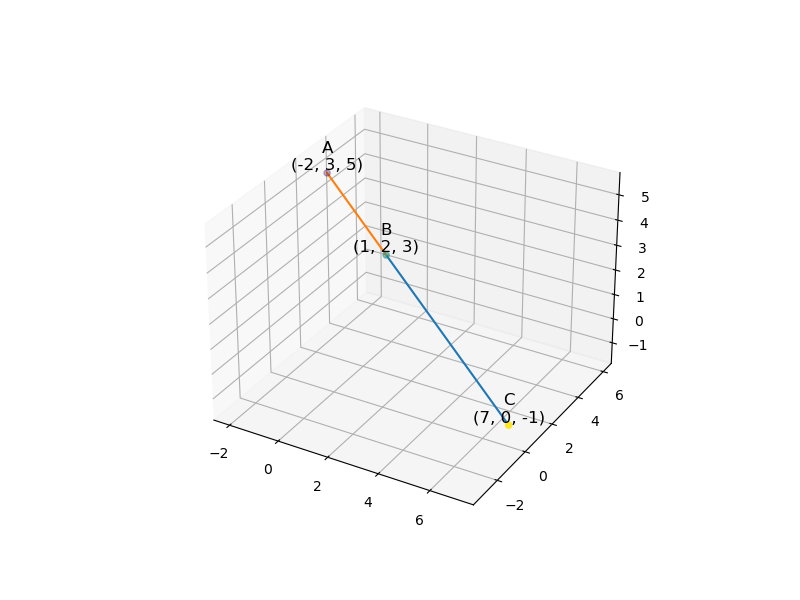
\includegraphics[width=\columnwidth]{figs/fig.png}
 \end{figure}
\end{frame}

\begin{frame}[fragile]
\frametitle{Python Code to find RREF of a 3x3 matrix}
\begin{minted}[bgcolor=bg, linenos, fontsize=\small, breaklines]{c}
import numpy as np

def rref(A):
    A = A.astype(float)
    rows, cols = A.shape
    r = 0
    
    for c in range(cols):
        if r >= rows:
            break
        
        max_row = np.argmax(np.abs(A[r:rows, c])) + r
        if A[max_row, c] == 0:
            continue
        
        A[[r, max_row]] = A[[max_row, r]]
        
        A[r] = A[r] / A[r, c]

\end{minted}
\end{frame}

\begin{frame}[fragile]
\frametitle{Python Code to find RREF of a 3x3 matrix}
\begin{minted}[bgcolor=bg, linenos, fontsize=\small, breaklines]{c}
        for i in range(rows):
            if i != r:
                A[i] -= A[i, c] * A[r]
        
        r += 1
    
    return A

A = np.array([[-2, 3, 5],
              [1, 2, 3],
              [7, 0, -1]])

rref_mat = rref(A)
print(rref_mat)
\end{minted}
\end{frame}

\end{document}
